




\tightsection{Evaluation}
\label{sec:eval}

In this section, we evaluate the performance of the GO system in real-world. 
The overall improvement is not impressive partly because the deployment is greatly constrained. The deployment only uses one content provider, and the content provider only enables CDN-level selection across three major CDNs which exhibit limited difference in their overall performance during the cause of our experiment. Moreover, the optimization must follow a traffic policy which dictates the total amount of traffic to each CDN. 

However, even with these constraints, we still see arguable improvement. 
%The initial bitrate selected by GO is close to the bitrate selected by the player logic during the period of playing and thus help player reaches its best sustainable bitrate with less bitrate swtiches.

\begin{packedenumerate}
    \item We see an overall 7\% reduction in buffering ratio, 4\% increase in average bitrate, and 16\% reduction in number of bitrate switches.
    \item We see buffering raito reduction of more than 20\% in several days when a major CDN is experiencing performance degradation.
    \item We show that the initial bitrate chosen by GO is 19\% closer to the dominant bitrate.
\end{packedenumerate}

\tightsubsection{Setup}
\label{subsec:eval_setup}

We evaluate the performance of GO on one content provider with short-form videos (5 minutes) on iOS device (both iPhone and iPad). 
HLS protocol is running on the iOS device and our GO system provides the initial CDN and bitrate, while Apple player employs adaptive 
bitrate switching algorithm. 

The results are collected from Jan 1st, 2014 to Jan 25th, 2014 (total of 25 days) with 26.1 million sessions (870K sessions on average per day).
There are three CDNs in this experiement, and 5 bitrate levels (from 700Kbps to 3.5Mbps). We evaluate two algorithms: {\it randomized} 
and {\it optimized} (by GO).

%\tightsubsection{Rebuffering Rate and Average Bitrate}
\tightsubsection{Quality improvement in real world}

Figure~\ref{subfig:buffering-and-bitrate} shows the performance improvement of GO over randomized algorithm on two quality metrics of
buffering rate and average bitrate over the 25-day period. The overall improvement over the entire 25-day period is 7\% reduction in buffering ratio and 4\% increase in 
average bitrate. The figure also shows that performance improvement varies by day, depending on how different the performance of each CDN. 
In fact, we noticed that, for this site, performance of multiple CDNs tend to become close to each other
during weekends where there CDNs are likely under-loaded, thus we see no noticeable improvement from GO in those days. 
On the other hand, on day 25, we noticed a big performance improvement of more than 20\%, after investigation,
we found that a major CDN was experiencing performance issues that lasts for more than one day. 

To further illustrate GO's ability to handle spatial and temporal variation, 
we look into some particular examples. Figure~\ref{fig:eval-case-study} shows two example days in which three CDNs performed differently: 
For example, in terms of buffering ratio, CDN3 was the best on Day A and CDN1 was the best on Day B. 
We can see that in both Day A and B, GO managed to outperform the best-performing CDN in both average bitrate 
and buffering ratio. This suggests that GO was not only looking for the globally best CDN, but also 
differentiated CDN performance in finer granular partition.

%\xil{add a spatial diversity graph}

\begin{figure*}[t!]
\centering
\subfigure[Buffering ratio and average bitrate]
{
  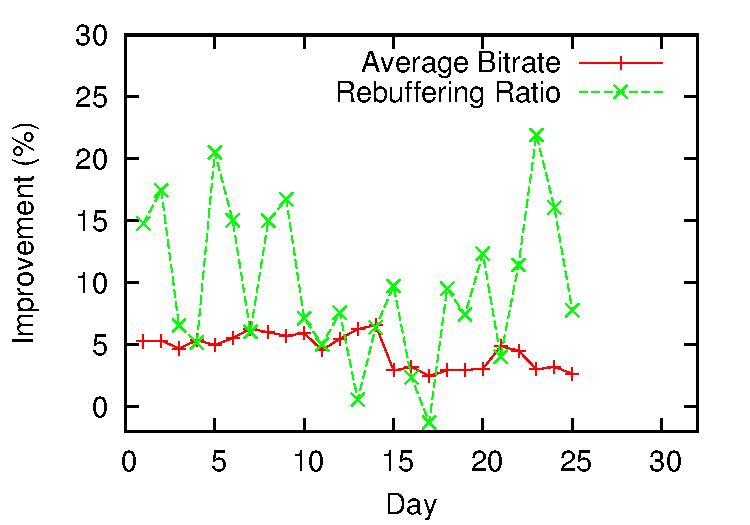
\includegraphics[width=0.3\textwidth] {figures/eval-perfimp.pdf}
  \label{subfig:buffering-and-bitrate}
}
\subfigure[Number of bitrate switches]
{
  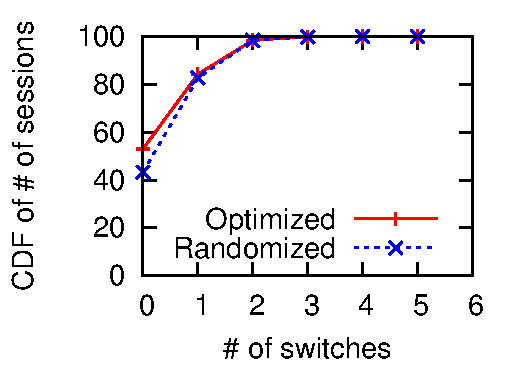
\includegraphics[width=0.3\textwidth] {figures/eval-reduceswitch.pdf}
  \label{subfig:reduce-switch}
}
\subfigure[Initial vs. dominant bitrate]
{
  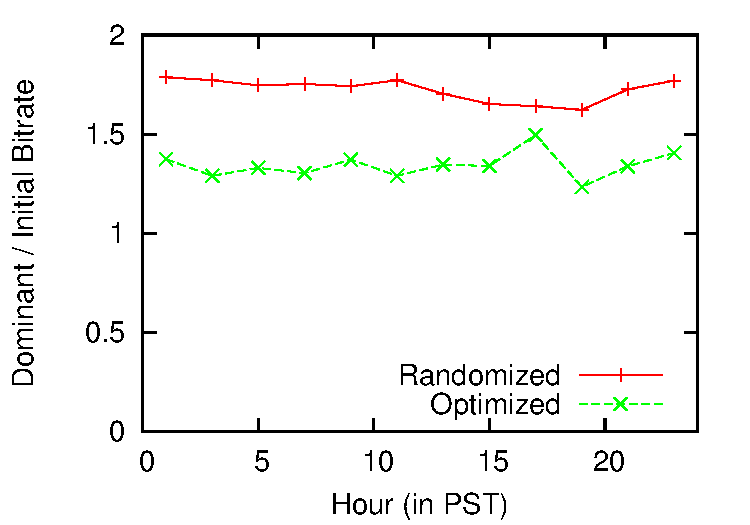
\includegraphics[width=0.3\textwidth] {figures/eval-initvsdom.pdf}
  \label{subfig:initvsdom}
}
\tightcaption{Performance Metrics and Improvement from GO}
\label{fig:perf-impr}
\end{figure*}

\begin{figure}[h!]
\centering
\subfigure[Buffering ratio]
{
	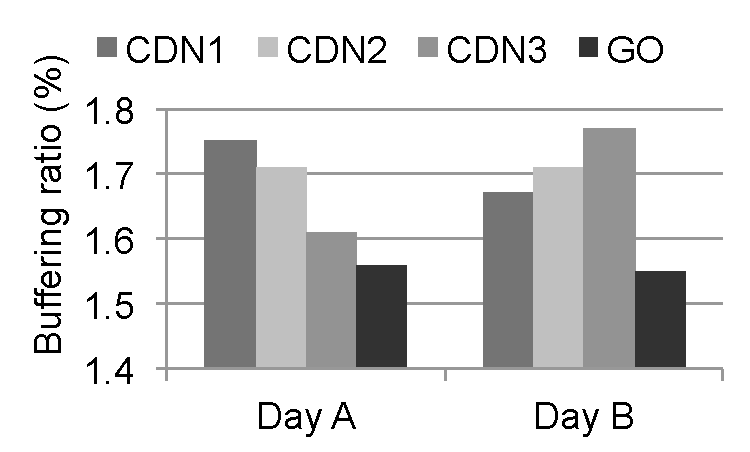
\includegraphics[width=0.24\textwidth]{figures/ab-testing-figures/bufferingratio-new.pdf}
	\label{subfig:eval-case-study:bufferingratio}
}
\hspace{-0.6cm}
\subfigure[Average bitrate (Kbps)]
{
	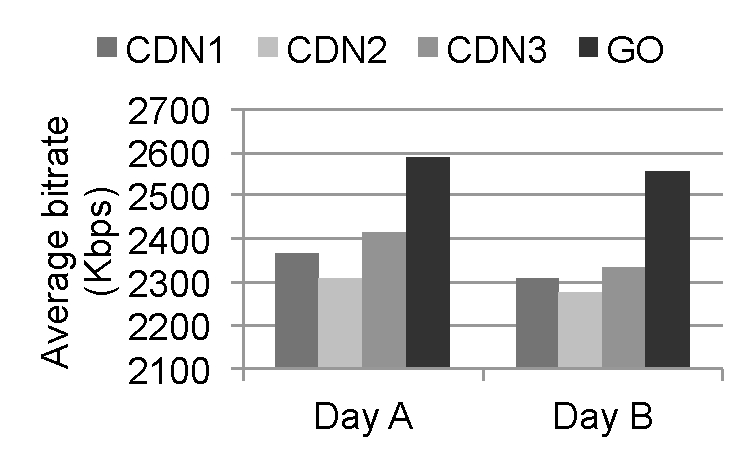
\includegraphics[width=0.24\textwidth]{figures/ab-testing-figures/averagebitrate-new.pdf}
	\label{subfig:eval-case-study:averagebitrate}
}
\tightcaption{Case study of two days: In both days, GO managed to improved the quality and give better quality than the best CDN.}
\label{fig:eval-case-study}
\end{figure}



\tightsubsection{Adaptive Bitrate Stability}

Previous research (e.g., ~\cite{user-adaptive,videoqoe}) shows that bitrate switching rate has an impact on video experience. In this section, we evaluate the adaptive 
bitrate switching behavior with and without GO. 

\myparatight{When Do Adaptive Bitrate Switches Happen?}
We first take a look at when do adaptive bitrate switches happen. Figure~\ref{fig:switch-time-dist} shows that the 
majority of switches happen at the beginning of the video plays, i.e., around 60\% of the switches 
happen within 20\% of the video duration. Switching behavior varies for different adaptive bitrate algorithms, and we do not 
claim such observation apply to all algorithms.

To account for viewers leaving in the middle of the video play, note that the x-axis is chosen as the percentage of actual 
video play duration instead of content length. 
In this figure, we include another content provider who provides long-formed content (one hour) on iOS platforms, and we have similar observations.

This suggests the importance of initial bitrate selection, through which viewers can have a smoother video playback experience.

\begin{figure}[h!]
\centering
 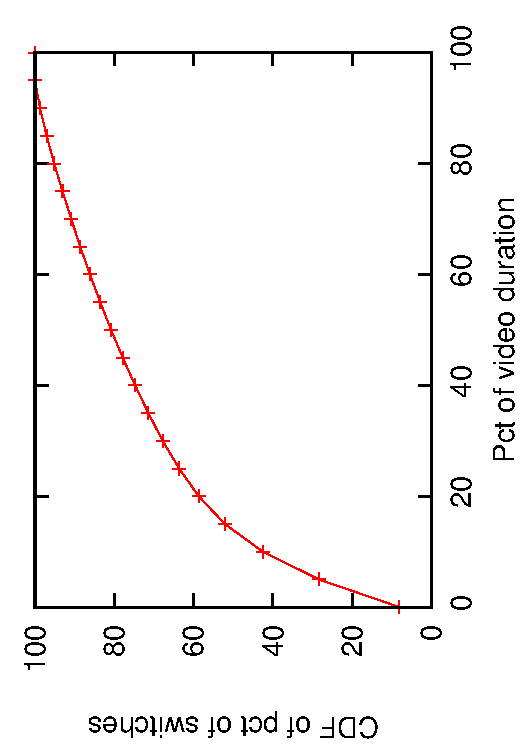
\includegraphics[width=0.4\textwidth] {figures/switch-time-dist.pdf}
\tightcaption{When Do Adaptive Bitrate Switches Happen}
\label{fig:switch-time-dist}
\end{figure}

\myparatight{Reducing Number of Bitrate Switch}
Next let us evaluate the switching stability by looking at the number of switches within the first minute of the video play.
We chose one minute because the videos are 5 minutes long and first minute account for 60\% of the switches (see Figure~\ref{fig:switch-time-dist}). 
Since HLS has 10 second video chunks, the maximum number of switches is 6 in this case.
Figure~\ref{subfig:reduce-switch} shows the number of bitrate switches for optimized and random decisions. 
Overall GO can reduce the number of switches by 16\%, and it also increases the number of non-switching-interrupted sessions 
(sessions that experience no switching) by 10\%.
It is possible the reason GO reduces the number of switches is shorter video plays, however, we observed engagement lift
(viewers watch longer because of better quality) at the same time of reduction in number of switches.

\myparatight{Dominant vs. Initial Bitrate}
Another metric we use to evaluate GO initial bitrate selection is the rate between dominant bitrate and initial bitrate. Dominant bitrate
is the bitrate that the sessions plays for the longest duration, and ideally this number should be 1. Figure~\ref{subfig:initvsdom} shows the 
ratio of initial bitrate to dominant bitrate. Overall GO is 19\% closer to the dominant bitrate than randomized bitrate selection. 
The figure also shows that for 60\% of the GO-optimized sessions, the initial bitrate selected by GO is almost the same as the dominant bitrate.
We would like to emphasize again that GO does not make the improvement at the price of engagement, and GO in fact improves engagement.

In summary, our early experience of GO in the real world suggests that it is a promising step towards the global control plane.
